\documentclass[dvipdfmx,autodetect-engine,titlepage]{jsarticle}
\usepackage[dvipdfm]{graphicx}
\usepackage{ascmac}
\usepackage{fancybox}
\usepackage{listings}
\usepackage{plistings}
\usepackage{itembkbx}
\usepackage{amsmath}
\usepackage{amssymb}
\usepackage{amsfonts}
\usepackage{svg}
\usepackage{url}
\usepackage{graphics}
\usepackage{listings,jvlisting}

\lstset{
  basicstyle={\ttfamily},
  identifierstyle={\small},
  commentstyle={\smallitshape},
  keywordstyle={\small\bfseries},
  ndkeywordstyle={\small},
  stringstyle={\small\ttfamily},
  frame={tb},
  breaklines=true,
  columns=[l]{fullflexible},
  numbers=left,
  xrightmargin=0zw,
  xleftmargin=3zw,
  numberstyle={\scriptsize},
  stepnumber=1,
  numbersep=1zw,
  lineskip=-0.5ex
}

\textheight=23cm
\renewcommand{\figurename}{図}
\renewcommand{\tablename}{表}
\newenvironment{code}
{\vspace{0.5zw}\VerbatimEnvironment  
\begin{screen} 
\baselineskip=1.0\normalbaselineskip
 \begin{Verbatim}}
{\end{Verbatim}
\baselineskip=\normalbaselineskip
 \end{screen}\vspace{0.5zw}} 

\title{情報理工学部 SNコース 3回\\
ワイヤレス通信システム\\
7th Week 演習問題}
\author{2600200443-6\\Yamashita Kyohei\\山下 恭平}
\date{Jun 12 2022}

\begin{document}

\maketitle

\section{}

matlabのソースコードとその結果を以下に示す。

\begin{lstlisting}[caption=hoge,label=fuga]

     
 gam = linspace(0,1);

 S = (1 + gam) ./ (1 - gam);
 
 M = 10 * log10 (((1 + S).^2) ./ (4 .* S));
 
 plot(S,M)
 xlim([1,10])

 xlabel('VSWR') 
 ylabel('M(db)') 


\end{lstlisting}

\begin{figure}[h]
  \centering
  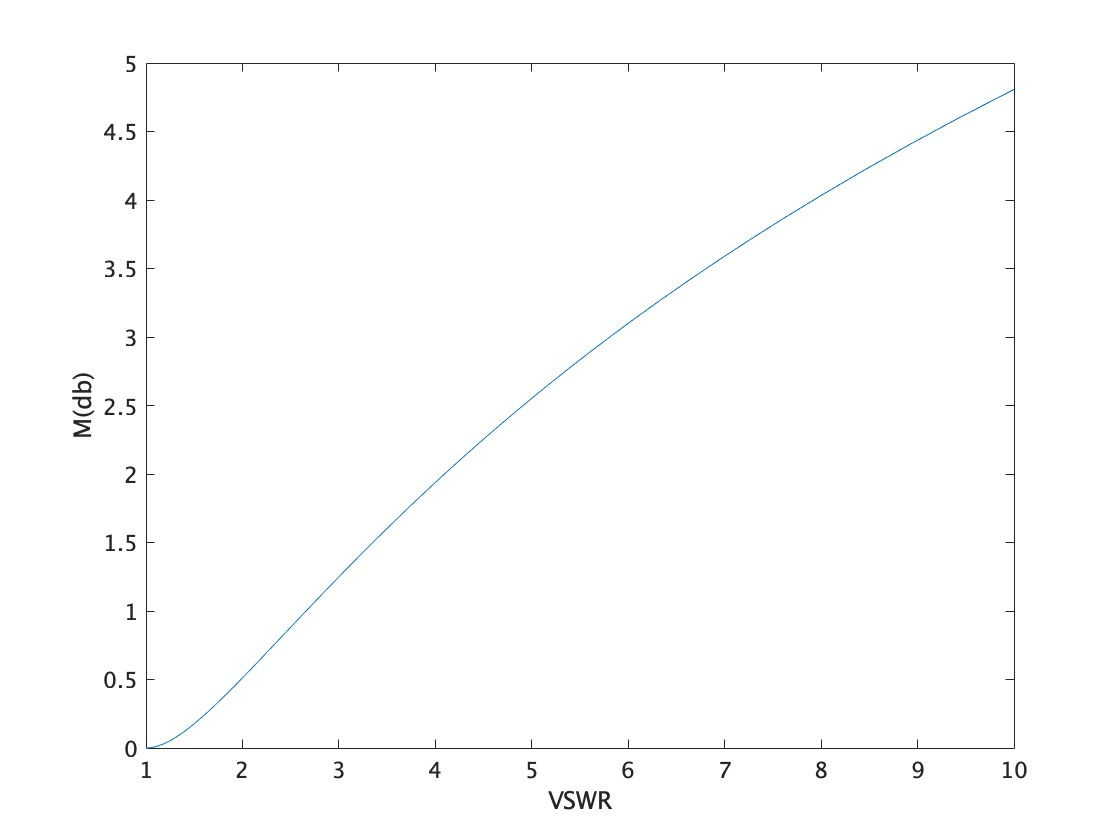
\includegraphics[scale=0.4]{VSW.jpg}
\end{figure}


\end{document}

